\section{Extraktion produktspezifischer Daten}
\label{sec:extraktion-produktspezifischer-daten}

Der Parser ist dafür verantwortlich die für den Vergleich relevanten Produktinformationen aus HTML-Dateien zu
extrahieren und zu normalisieren.
Dies ist ein sehr wichtiger Schritt, da die Qualität der extrahierten Werte die Ergebnisse der Matcher-Komponente
stark beeinflussen könnte.

\subsection{Die technischen Anforderungen an den Parser}
\label{subsec:technische-anforderungen-parser}

Die Herausforderung der Parser-Komponente besteht hauptsächlich darin, das heterogene Informationsschemata der
verschiedenen Shops in ein homogenes, normalisierten Schema zu bringen.

Im Detail geht es darum, zu jedem Angebot den Titel, die Produktbeschreibung, den Preis, die Marke, die Kategorie,
die Produktbilder sowie weitere eindeutige Merkmale im Format von idealo zu erfassen.
Diese eindeutigen Merkmale sind zum Beispiel die standardisierte EAN (Europäische Artikelnummer), HAN (Händler
Artikelnummer) und SKU (Stock keeping unit -- eine shop-spezifische Kennung).

Da die Crawler-Komponente sehr viel Zeit benötigt um alle Seiten zu erfassen, spielt der Zeitfaktor für den Parser
keine große Rolle.
Eine schnelle Verarbeitung der Seiten ist dennoch wünschenswert.

Es gilt sowohl eine hohe Trefferzahl als auch eine hohe Genauigkeit zu erzielen, damit die  Ergebnisse des Parsers
als zuverlässig eingestuft werden.
Je genauer die Ergebnisse des Parsers im Format von idealo vorliegen, desto einfacher sollte der Vergleich durch die
Matcher-Komponente werden.

\subsection{Die Positionsbestimmung der Produktattribute}
\label{subsec:herangehensweisen}

Die eigentliche Schwierigkeit der Datenextraktion liegt in der Bestimmung der Stellen, an denen die gewünschten
Informationen stehen.
Es gibt grundsätzlich zwei Möglichkeiten, wie man die Informationen aus den Angeboten extrahieren kann.
Wir haben zwischen dem shop-unspezifischen und den shop-spezifischen Ansatz unterschieden.

Die Initiative Schema.org hat bereits 2011\footnotemark eine erste Lösung für den \textit{shop-unspezifischen} Ansatz
entwickelt.
\footnotetext{\url{https://schema.org/docs/about.html}}
Schema.org hat einen Standard entwickelt, den Webseitenbetreiber nutzen können, um bestimmte Daten zu markieren.
Shopbetreiber können zum Beispiel die Produktrezensionen, den Preis oder auch den Produktnamen hervorheben.
Große Suchmaschinenanbieter wie Google, Microsoft oder Yandex können dadurch sehr einfach relevante Informationen
direkt in den Suchergebnissen anzeigen.
Die Angebote der Onlinehändler werden somit besser dargestellt.

Laut einer Schätzung von idealo verwenden rund 40\% der Shops diesen Standard.
Diese Herangehensweise bezeichnen wir als shop-unspezifischen Ansatz, da man generische Regeln verwenden kann,
um die standardisierten Informationen zu erfassen.
Eine Lösung zum Auslesen dieser Informationen ist recht einfach und schnell umsetzbar.
\\
\\
Alternativ zum shop-unspezifischen Ansatz gibt es die \textit{shop-spezifische} Herangehensweise, d.h.\ dass für jeden
Onlineshop individuell angepasste Spezifikationen für die Extraktion erstellt werden.
Die Regeln des shop-spezifischen Ansatzes bilden eine Übermenge des shop-unspezifischen Ansatzes.

Die Umsetzung dieser Variante ist anspruchsvoller, da diese Spezifikationen zunächst erstellt werden müssten.
Wir nehmen jedoch an, dass durch diesen Ansatz sowohl die Trefferquote als auch die Präzision des Parsers
im Vergleich zu dem shop-unspezifischen Ansatz erhöht werden.

Zu Beginn haben wir erste Versuche basierend auf dem Schema.org-Standard unternommen.
Leider haben wir schnell feststellen müssen, dass die Spezifikation oft nicht richtig eingehalten wurden.
Dies hat die Qualität der extrahierten Daten stark verringert.
Auch bei anderen Standards, welche bei der Strukturierung von Produktdaten im Internet helfen sollen, wie zum Beispiel
JSON-LD\footnotemark (W3C) und das Open-Graph-Protokoll\footnotemark (Facebook), konnten wir ähnliche Beobachtungen
machen.
\footnotetext{\url{https://json-ld.org/}}
\footnotetext{\url{http://www.ogp.me/}}

Wir haben uns deshalb gegen den shop-unspezifischen Ansatz entschieden.

\subsection{Die Annahmen für die Umsetzung der shop-spezifischen Methode}
\label{subsec:annahmen}

Für die Umsetzung der Parser-Komponente haben wir zwei Annahmen getroffen, welche die Konzeption des Algorithmus
beeinflusst haben.

Wir nehmen an, dass jeder Shop aufgrund der Vielzahl von Angeboten ein Content Management System (CMS) zur Verwaltung
seiner Angebote verwendet.
Daraus resultierend gehen wir davon aus, dass sich durch die Verwendung eines CMS die Struktur der Angebote eines Shops
ähnelt und diese erlernt werden kann.

Außerdem erwarten wir, dass idealo aufgrund der Vertragsvereinbarungen für die zu untersuchenden Shops bereits
eine gewisse Menge an Angeboten besitzt und die Produktattribute nicht manipuliert wurden.

\subsection{Die zwei Schritte der Datenextraktion}
\label{subsec:grundidee}

Für die nachfolgenden Erklärungen werden die beiden Begriffe Regel und Selektor definiert.
Eine \textit{Regel} ist eine Sammlung von Selektoren für eine bestimme Produkteigenschaft.
Jeder \textit{Selektor} dieser Regel stellt eine Wegbeschreibung durch das HTML-Dokument dar.
Er führt zu dem gewünschten Element, aus dem das Produktattribut extrahiert werden soll.
\\
\\
Der grobe Ablauf der shop-spezifischen Datenextraktion kann in zwei Phasen untergliedert werden:
\begin{enumerate}
    \item Die Generierung der shop-spezifischen Extraktionsregeln/ Spezifikation
    \item Die Anwendung der Regeln auf die vom Crawler erzeugten Seiten
\end{enumerate}

In der ersten Phase sollen die Regeln, welche für die Extraktion benötigt werden, mit Hilfe der Daten von idealo
angelernt werden.

Die generierten Regeln werden in der zweiten Phase angewendet, sodass zu jeder Produkteigenschaft genau ein Wert
zugeordnet wird.
Für jede gecrawlte Seite werden die extrahierten Produktattribute abgespeichert.

Die Logik der beiden Phasen spiegelt sich in der Architektur des Parsers wieder.
Dieser besteht aus dem Shop Rules Generator (SRG), der Parser-Komponente und dem URL-Cleaner.
Auf die Notwendigkeit des URL-Cleaners und dessen Funktionsweise wird in Kapitel~\ref{subsec:urlcleaner} eingegangen.
Die resultierende Architektur ist in Abbildung~\ref{abb:architektur-parser} abgebildet.

\begin{figure}[H]
    \centering
    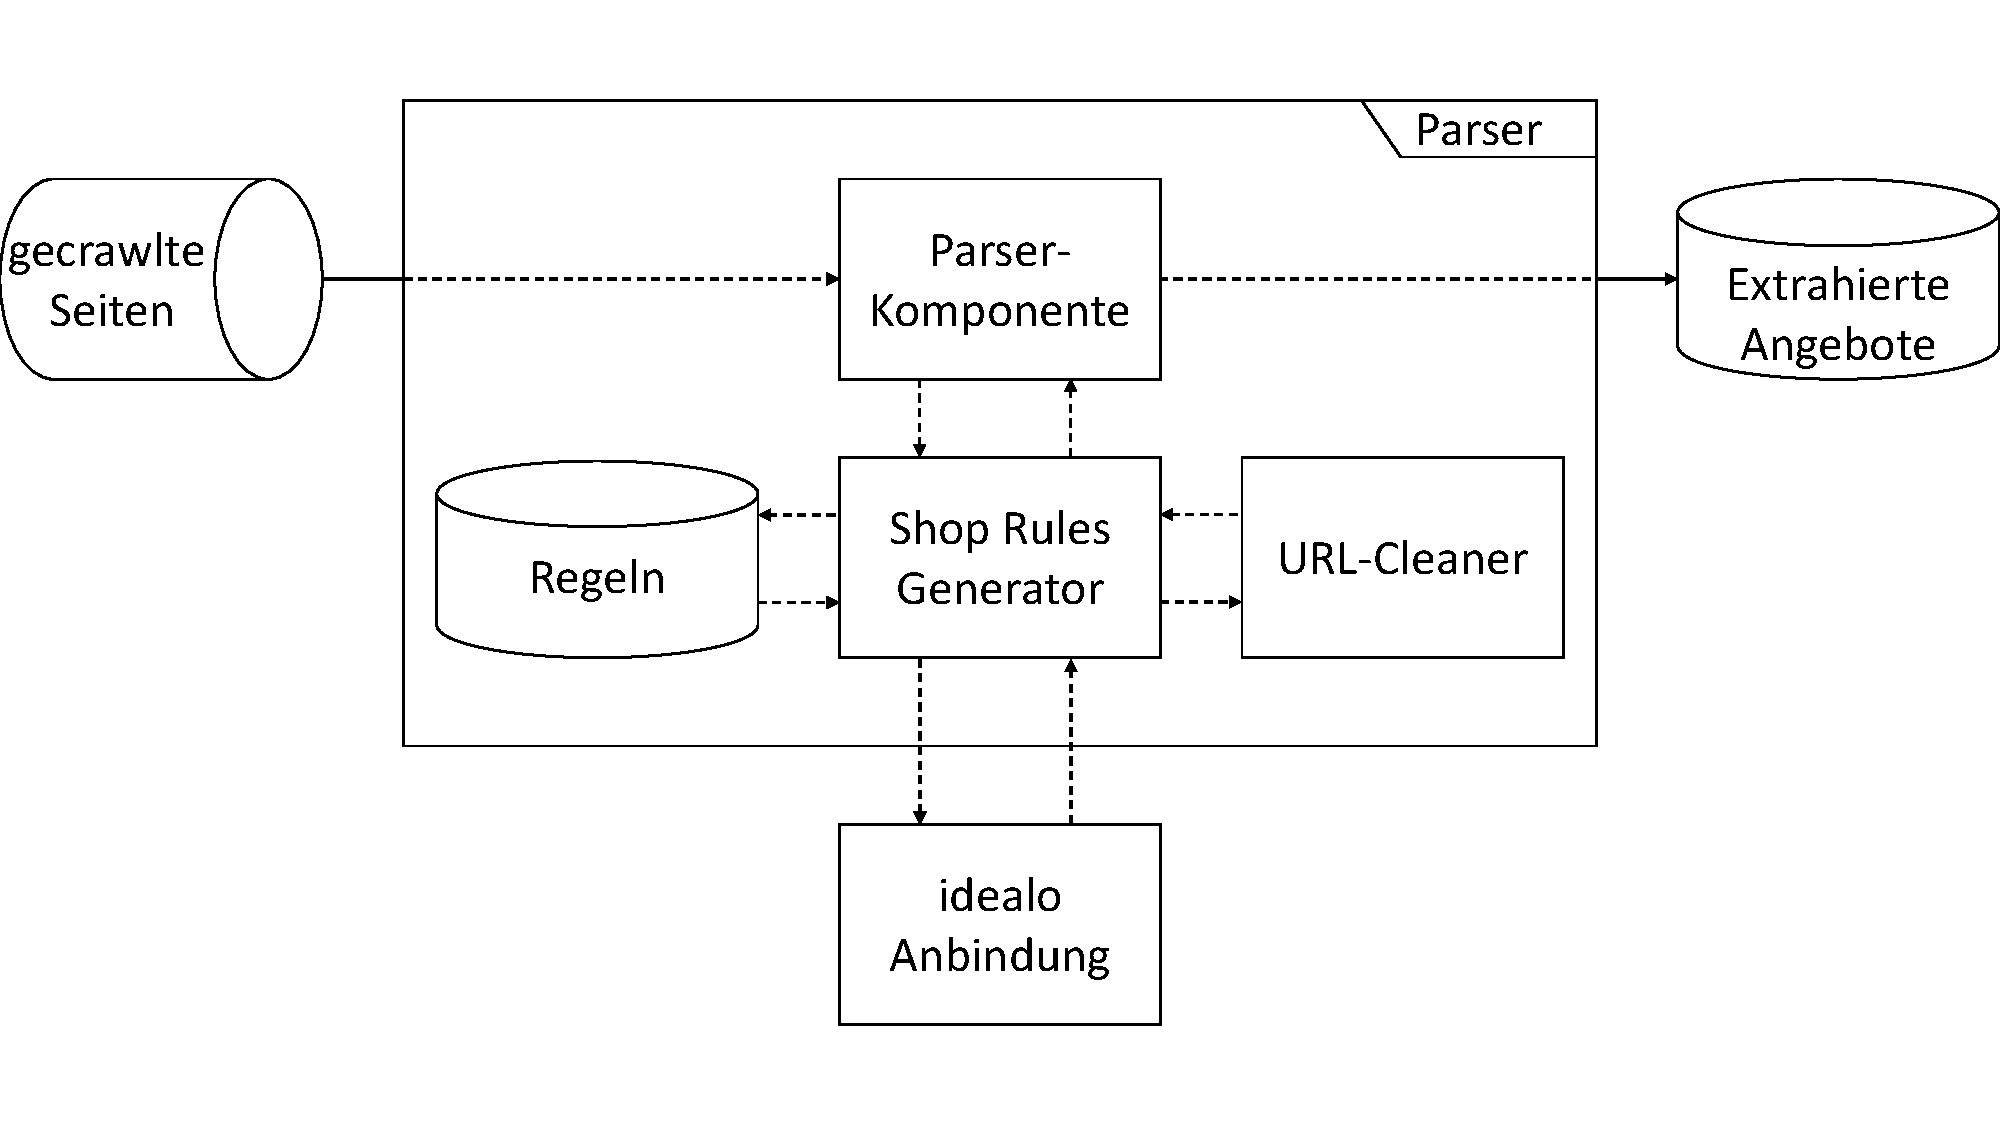
\includegraphics[width=13cm, trim=0 1.7cm 0 1.7cm, clip]{resources/Architektur-Parser.pdf}
    \caption{Architektur des Parsers}
    \label{abb:architektur-parser}
\end{figure}

\subsection{Die Funktionsweise der Parser-Komponente}
\label{subsec:funktionsweise-parser}

Die Parser-Komponente erhält ihre Eingaben, indem sie Nachrichten aus einer Queue konsumiert.
Eine Nachricht enthält eine vom Crawler heruntergeladene Webseite.
Der Crawler sendet zusätzlich zu jeder Seite, die Webadresse und die Identifikationsnummer des zugehörigen Shops mit.
Nach dem Erhalt einer Nachricht, lädt der Parser vom Shop Rules Generator (SRG) die Extraktionsregeln für den
entsprechenden Shop.

Sollten die Regeln noch nicht existieren, wartet der Parser solange, bis diese vom SRG erstellt wurden.
Sobald der Parser die Regeln empfangen hat, werden die Produktattribute aus der gecrawlten Seite extrahiert.
Zum Schluss werden diese in einer Datenbank normalisiert abgespeichert.

Der Matcher greift später auf diese Datenbank für den Vergleich zu.

\subsection{Die Funktionsweise des Shop Rules Generators}
\label{subsec:funktionsweise-srg}

Der Shop Rules Generator (SRG) gibt auf Anfrage die Regeln für einen beliebigen Shop zurück.
Sollten diese noch nicht existieren, werden sie generiert.
Während des Generierungsprozesses durchläuft der SRG mehrere Schritte.

Zuerst werden eine bestimmte Anzahl von Angeboten aus der idealo-Datenbank geladen.
Dies erfolgt über einen von idealo zur Verfügung gestellten API-Endpoint, welcher den Datenbankzugriff über eine
REST-Schnittstelle kapselt.
Dies hat den Vorteil, dass wir die Infrastruktur von idealo nutzen können und keine Kopie der Angebotsdaten
lokal speichern müssen.

Zu jedem dieser Angebote liegen die Webadresse, sowie die Informationen über die in
Kapitel~\ref{subsec:technische-anforderungen-parser} genannten Produktattribute vor.
Außerdem wird für jedes Angebot das dazugehörige HTML-Dokument heruntergeladen.

Um die Server der Onlineshops nicht durch zu viele simultane Anfragen zu strapazieren, wird nach jedem
Download eine fest definierte Zeit gewartet.

Für die Menge der heruntergeladenen HTML-Dokumente ist somit bekannt, um welche Angebote es sich handelt und welche
konkreten Produktattribute erwartet werden.

Dieses Wissen wird für das Anlernen der Regeln genutzt.
Dazu werden die Werte aller Produkteigenschaften in dem HTML-Dokument gesucht.
Für jedes Vorkommnis eines Produktattributes wird ein Selektor erstellt, der den Fundort referenziert und einer Regel
zugeordnet.

Nachdem alle Regeln gesammelt wurden, wird eine finale Regelmenge bestimmt, welche in der Regeldatenbank gespeichert
und bei zukünftigen Anfragen direkt zurückgegeben wird.

\subsection{Der URL-Cleaner}
\label{subsec:urlcleaner}

Manche Onlinehändler manipulieren vor der Übermittlung ihrer Angebote an idealo die Links zu deren Angeboten.
Sie fügen zu den regulären Webadressen Trackinginformationen hinzu.
Mit Hilfe dieser Trackinginformationen können sie nachvollziehen, welche Kunden durch idealo auf deren Seite gelandet
sind.

Dies ist für die Shopbesitzer sehr wichtig, da sie somit die CPC-Abrechnung von idealo kontrollieren können.
Die im Rahmen der Anlernphase getätigten Webseitenaufrufe könnten diese Statistiken jedoch verfälschen.
Für idealo ist es deshalb sehr wichtig, dass die Trackinginformationen vor dem Aufruf der Website entfernt werden.
\\
\\
Dazu haben wir die URL-Cleaner-Komponente entwickelt, welche Adressen mit Trackinginformationen als Eingabe erwartet und
bereinigt zurück gibt.

Wir haben zwei mögliche Verfahren entdeckt, wie die Trackinginformationen in Angebotlinks eingefügt werden können.
Dies ist sowohl über Weiterleitungen als auch URL-Parameter möglich.
Der URL-Cleaner wendet deshalb zwei Strategien sukzessive an, um die Trackinginformationen zu entfernen:
\\
\\
Die erste Strategie bereinigt die URL von Weiterleitungen.
Dabei gibt es zwei mögliche Verfahren der Weiterleitungsdienste:

Beim ersten Verfahren leitet der zwischengeschaltete Server den Besucher anhand der mitgesendeten URL-Parameter auf
die korrekte Seite weiter.
Die ursprüngliche URL ist hierbei somit bereits in der Modifizierten enthalten.

Das zweite Verfahren ist etwas schwieriger, da anstatt der Ziel-Adresse lediglich ein kryptischer String mitgesendet
wird.
Die Weiterleitung ist erst nach der serverseitigen Zuordnung des kryptischen Strings zur tatsächlichen Adresse möglich.

In der Tabelle~\ref{tab:redirect} sind zwei Beispiele abgebildet, wie solche Weiterleitungen aussehen könnten.
Eine Mischform der beiden Varianten ist ebenfalls möglich.

\begin{table}[h]
    \centering
    \begin{tabular}{ l | l }
        URL-Parameter                 &   cptrack.com/?redir=\textbf{www.shop.de/product1}\\
        krypt.\ Identifikationsstring   &   bit.ly/\textbf{2Kqyrz2}
    \end{tabular}
    \caption{Beispiele der Weiterleitungsverfahren}
    \label{tab:redirect}
\end{table}

Für die Bereinigung von Weiterleitungen wird die übergebene URL zunächst encodiert.
Anschließend wird die Root-Url des Shops in der encodierten URL gesucht und alles davor entfernt.
Für die Weiterleitungen, welche kryptische Identifikationsstrings verwenden, haben wir keine zufriedenstellende Lösung
finden können.
Allerdings wird dieser Fall durch das Fehlen der Root-URL des Shops in der encodierten URL erkannt.

\begin{table}[h]
    \centering
    \begin{tabular}{ c }
        http://www.shop.de/product?\textbf{partner=idealo}?pid=96
    \end{tabular}
    \caption{URL mit parameterbasierten Trackinginformationen}
    \label{tab:trackparameter}
\end{table}

Die Tabelle~\ref{tab:trackparameter} zeigt eine Beispiel-URL mit parameterbasierten Trackerinformationen.
Dabei können ebenfalls Parameter enthalten sein, welche nicht für das Tracking verwendet werden.

Um die parameterbasierten Trackerinformationen zu entfernen, werden alle Schlüssel-Wert-Parameterkombinationen
gelöscht, deren Schlüssel in einer vorher angelegten Liste vorkommen.
Diese Liste enthält alle Tracker-Schlüsselnamen, die bei einer manuellen Recherche über mehrere hundert Shops
häufiger vorgekommen sind.

Nachdem beide Strategien angewandt wurden, wird die bereinigte URL zurückgegeben.

\subsection{Die Erstellung von Selektoren}
\label{subsec:erstellen-von-selektoren}

Im nachfolgenden wird darauf eingegangen, wie die Selektoren während der Regelerstellung erzeugt werden.
Für die Erläuterung werden Begriffe wie \textit{Document Object Model (DOM)}, \textit{Element} oder \textit{Tag} aus
dem Kontext der hierarchiebasierten Sprache HTML verwendet.
Bei Bedarf kann der entsprechende Wikipedia-Artikel\footnotemark für einen kurzen Einstieg gelesen werden.
\footnotetext{\url{https://de.wikipedia.org/wiki/Hypertext_Markup_Language}}

Um einen Selektor zu erstellen muss zunächst ein konkretes Element der DOM-Hierarchie bestimmt werden.
Dieses wird von dem SRG in einem vorherigen Schritt ermittelt und stellt den Fundort für ein gewünschtes
Produktattribut dar.

Es wird zwischen den folgenden drei Knotentypen unterschieden: Textknoten, Beschreibungsknoten und Datenknoten.

\textit{Textknoten} sind Elemente, bei denen das gewünschte Produktattribut innerhalb eines Tag-Paars steht.
Das Attribut ist somit ein sichtbarer Bestandteil der Browservisualisierung.

Zu den \textit{Beschreibungsknoten} gehören die Elemente, bei denen das gesuchte Produktattribut innerhalb der
Attributliste des Elementes vorkommt.
Dieses Attribut ist im Gegensatz zum Textknoten kein sichtbarer Bestandteil der Visualisierung.

In dem Beispiel~\ref{exa:text-and-beschreibungsknoten} ist jeweils ein kurzes Beispiel für beide Typen aufgeführt.
Der gesuchte Wert ist in diesem Fall die Produkteigenschaft EAN mit dem Produktattribut 9332721000108.

\lstset{
    escapeinside={(}{)},
    frame=single,
    language=html,
    xleftmargin=.25in,
    xrightmargin=.25in
}
\begin{lstlisting}[
    caption=Beispiele für einen \circled{1} Textknoten und einen \circled{2} Beschreibungsknoten,
    captionpos=b,
    label=exa:text-and-beschreibungsknoten]
    <div id='product-details'>
        (\circled{1}) <span>9332721000108</span>
    </div>
    (\circled{2}) <meta itemprop='gtin13' content='9332721000108'>
\end{lstlisting}

Die Selektoren der beiden Knotentypen sind ähnlich aufgebaut und bestehen jeweils aus einem CSS-Selektor.
Der Aufbau des CSS-Selektors erfolgt analog zu der "Copy selector"-Funktion der Chrome-Entwicklertools.
Der Selektor für einen Beschreibungsknoten speichert zusätzlich einen Schlüssel, um das korrekte Elementattribut
auszulesen.

Wir haben festgestellt, dass viele Internetshops Javascript auf ihrer Webseite verwenden.
Oftmals sind in diesem Fall die produktspezifischen Daten bereits in einer strukturierten Form im Javascript
als Objekt in der Javascript Objekt Notation (JSON) enthalten.
In dem Beispiel~\ref{exa:datenselektor} ist ein solches Skript vereinfacht dargestellt.

\lstset{
    escapeinside={(}{)},
    frame=single,
    language=javascript,
    literate=%
        {Ö}{{\"O}}1
        {Ä}{{\"A}}1
        {Ü}{{\"U}}1
        {ß}{{\ss}}1
        {ü}{{\"u}}1
        {ä}{{\"a}}1
        {ö}{{\"o}}1,
    showstringspaces=false,
    xleftmargin=.25in,
    xrightmargin=.25in
}
\begin{lstlisting}[
    caption=Javascript\, dass produktspezifische Informationen enthält,
    captionpos=b,
    label=exa:datenselektor]
    <script>
        var gtmGuaranteeProduct1 = {
            "name":"Versicherung für 2 Jahre",
        };
        var product2400462 = {
            "name":"Product",
            "ean":"9332721000108"
        };
    </script>
\end{lstlisting}

Der Aufbau eines Pfades durch eine Hierarchie hat beim DOM sehr gut funktioniert.
Wir wollen daher das selbst Prinzip auf das Script-Tag anwenden.
Dazu muss die Struktur des Javascripts in eine hierarchische Form gebracht werden.

Der resultierende \textit{Datenselektor} besteht aus drei Teilen.
Einer davon ist, genau wie die anderen beiden Selektortypen, ein CSS-Selektor.
Dieser CSS-Selektor zeigt zu dem entsprechenden Script-Tag im DOM .
Um innerhalb des Javascriptes das richtige JSON-Objekt zu finden, wird ein Pfad verwendet, welcher durch die
verschiedenen Code-Blöcke navigiert.
Der Block-Pfad wird durch eine Tiefensuche durch die verschachtelten Blöcke erstellt.
Ein Block wird durch \textit{\{} und \textit{\}} markiert.
Der Pfad zeigt auf einen Block, welcher als JSON interpretiert werden kann.
Innerhalb dieses JSON-Objektes wird mittels des standartisierten JSON-Path navigiert.
Dieser ist einem XPath ähnlich.

Der resultierende Datenselektor sieht wie in Tabelle~\ref{tab:datenselektor} dargestellt aus.

\begin{table}[h]
    \centering
    \begin{tabular}{ l | l }
        CSS-Selektor &  html > head > script:nth-of-type(1)\\
        Block-Pfad   &  -> 1\\
        JsonPath     &  \$['ean']
    \end{tabular}
    \caption{Datenselektor für Beispiel~\ref{exa:datenselektor}}
    \label{tab:datenselektor}
\end{table}

\subsection{Die Trimming-Funktion}
\label{subsec:trimming-funktion}

Eine generische Verbesserung, welche auf alle Selektoren angewendet werden kann ist die Trimming-Funktion.
Häufig stehen vor und nach den gesuchten Produktattributen andere irrelevante Informationen.
Vor der gesuchten EAN steht zum Beispiel der String 'EAN:\textvisiblespace', welcher entfernt werden soll.
Die generierten Regeln enthalten Informationen, wie viele Stellen links oder rechts abgeschnitten werden sollen.
Diese bezeichnen wir als Left-Cut und Right-Cut.
Sollte vor der gesuchten EAN immer derselbe String stehen, so gibt es keine Streuung in den Left-Cut-Werten.
Wenn es sich bei dem Produktattribut um die Beschreibung handelt und diese durch manuelle Änderungen von idealo von
denen der Webseite abweicht, so gibt es eine starke Streuung der Left- und Right-Cut-Werten.

\subsection{Das Bewertungssystem für die Selektoren}
\label{subsec:bewertungssystem}

Durch die verschiedenen Möglichkeiten Selektoren zu generieren sowie durch die Trimmingfunktion werden sehr viele
Selektoren erstellt.
Die gewonnene Flexibilität ist zwar gewollt, hat jedoch den Nachteil das ein "Rauschen" der extrahierten Daten entsteht.
Dieses "Rauschen" entsteht dadurch, dass nun sehr viele Daten extrahiert werden.
Allerdings ist nun nicht mehr bekannt, welche extrahierten Informationen korrekt oder falsch sind.
Um diesen Fakt entgegenzuwirken wurde ein Bewertungssystem für Selektoren eingeführt.
Nachdem alle Selektoren mit Hilfe der Angebote von idealo angelernt wurden, wird jedem Selektor ein Qualitätsindex
zugewiesen.
Es wird dafür noch einmal über die Angebote, welche zum Anlernen genutzt wurden, von idealo iteriert.
Für jedes Angebot werden alle Selektoren angewandt und die extrahierten Produktattribute mit denen von idealo
verglichen.
Sollten die Werte identisch sein, so wird der Qualitätsindex des Selektors erhöht.
Wenn die Werte unterschiedlich sind, so wird der Index verringert.
Ein Ausnahmefall bildet der leere String: Wird dieser als extrahierter Wert zurückgegeben, so bleibt der
Qualitätsindex unverändert.
Wir haben uns dafür entschieden, da man den leeren String von einem unerwünschten bzw.\  falschen Wert unterscheiden
kann.
Dies soll nicht so schwer ins Gewicht fallen, wie eine fehlerhaft extrahierte Information, da man später beim
Extraktionsvorgang genau diesen Fall unterscheiden kann.
Bevor die Regeln mit dem Qualitätsindex in der Datenbank abgespeichert werden, werden diese auf den
Intervall 0 bis 1 normalisiert.
Alle Regeln mit einem normalisierten Index unter einem bestimmten Schwellwert werden verworfen.
Die Parser-Komponente verwendet diesen Qualitätsindex, um aus allen gefundenen Werten den besten zu ermitteln.
Dazu gruppiert sie nach den extrahierten Werten und summiert den Qualitätsindex.
Für jedes Produktattribut wird somit nur das beste Ergebnis gespeichert.